% =============================================================
%  Chapter 6 — Experimental Evaluation and Failure Analysis
% =============================================================

\chapter{Experimental Evaluation and Failure Analysis}
\label{chap:experiments}

\providecommand{\Ham}{\mathcal{H}}
\providecommand{\Potential}{\mathcal{R}}
\providecommand{\PhaseState}{z}
\providecommand{\Pos}{q}
\providecommand{\Mom}{p}
\providecommand{\Mass}{\mathrm{M}}

% -----------------------------------------------------------------------
\section{Experimental Questions}
\label{sec:ch6:questions}
% -----------------------------------------------------------------------

This chapter validates both stages empirically and probes
the failure modes that motivated the enrichment hierarchy.
Every result subsection is organized around one of four questions:

\begin{enumerate}
  \item[\textbf{Q1.}]
        How well does the geometry-only learner (Stage~1, Ch.~\ref{chap:grlsnam})
        perform under local sensing alone, relative to classical planners
        and standard RL baselines?
  \item[\textbf{Q2.}]
        What does material-aware structure (Stage~2, Ch.~\ref{chap:material})
        add beyond geometry? How much risk reduction does the richer
        hierarchy provide?
  \item[\textbf{Q3.}]
        Which specific added components drive the improvement?
        (Ablation study organized around the enrichment hierarchy of
        Ch.~\ref{chap:hierarchy}.)
  \item[\textbf{Q4.}]
        Which failure modes are resolved, and which remain?
        What does the remaining oracle gap look like?
\end{enumerate}

% -----------------------------------------------------------------------
\section{Datasets, Environments, Metrics, and Protocol}
\label{sec:ch6:setup}
% -----------------------------------------------------------------------

\subsection{Geometry-Only Benchmark}
\label{subsec:ch6:geom_bench}

\paragraph{Environments.}
Two benchmarks are used for Stage~1 evaluation.

\textbf{Hyperelastic ring navigation.}
The primary geometry benchmark is a deformable hyperelastic ring robot
in procedurally generated cluttered workspaces of size $[0,L]^2$.
Each workspace contains randomly sampled circular obstacles spanning
bottlenecks, zig-zag corridors, and cul-de-sacs.
Start–goal pairs are sampled such that a deformable ring has a
collision-free path while a rigid disc of comparable size may not,
stressing shape adaptation.
Three data splits are used:
\begin{itemize}
  \item \textbf{Train:} 2000 environments, matched obstacle statistics.
  \item \textbf{Test-ID:} 400 environments, same statistics.
  \item \textbf{Test-OOD:} 400 environments, shifted gap width and
        obstacle density.
\end{itemize}

\textbf{Dungeon point-agent navigation.}
The secondary geometry benchmark uses dungeon layouts from~\citet{liang2023context}.
A \texttt{StagewiseSensor} provides the current stage exit; an
\texttt{ObstacleExtractor} fits circular obstacles to locally visible
wall segments.
This benchmark isolates the learning formulation from deformability.

\paragraph{Sensing.}
In both environments the agent observes only the local window
$\mathcal{W}(\vec{q}_t)$ of half-width $\hat{d}$ centred at the
current pose.
The mapping ratio $\rho_{\mathrm{map}}$ (eq.~\eqref{eq:ch3:map_ratio})
measures sensing economy.

\subsection{Material-Aware Benchmark}
\label{subsec:ch6:mat_bench}

\paragraph{Dataset.}
Stage~2 evaluation uses the \textbf{DFC2018 Houston aerial dataset},
a large-scale hyperspectral+LiDAR scene containing terrain classes with
heterogeneous material risk:
water bodies ($\tilde{r} = 1.0$, hard hazard),
major highways and railways ($\tilde{r} = 0.8$--$0.9$, hard hazard),
low vegetation ($\tilde{r} = 0.15$, soft risk),
and impervious surfaces ($\tilde{r} \approx 0$, safe).
The oracle material map $Z^{(2)}$ provides ground-truth
$\tilde{r}(\vec{c})$ and $\phi(\vec{c})$ at all positions.

\paragraph{Episodes.}
300 canonical episodes with fixed start–goal pairs are generated, with
guaranteed geometry-feasible paths from $Z^{(1)}$ (LiDAR-derived
occupancy).
The split is 200 training / 40 validation / 60 test, stratified to
ensure representation of high-risk, low-risk, and mixed-terrain routes.
The 20 test episodes reported in the main results table are a
held-out high-risk subset in which baselines are most challenged.

\paragraph{Oracle access.}
In the current chapter, $\tilde{r}$ and $\phi$ are provided
as oracle inputs (Setting~2 of the thesis scope).
LiDAR geometry is used for obstacle extraction and waypoint scaffolding;
the material maps augment this with risk information.
\subsection{Metrics}
\label{subsec:ch6:metrics}

We evaluate performance using the following metrics. \textbf{Success rate} (\%) measures the fraction of episodes that reach within $\epsilon_{\mathrm{goal}} = 0.5\,\text{m}$ of the goal. \textbf{Terminal goal distance} (m) is the final Euclidean distance $\|\vec{q}_T - \vec{g}\|$, averaged over episodes. \textbf{Path length} (m) is defined as $\sum_t \|\vec{q}_{t+1} - \vec{q}_t\|$.

We additionally report \textbf{SPL} (success-weighted path length),\\
$\frac{1}{N}\sum_i S_i \cdot L_{\mathrm{ref},i} / \max(P_i, L_{\mathrm{ref},i})$,
where $L_{\mathrm{ref}}$ is the A$^*$ reference path length. Safety is quantified via \textbf{minimum clearance} (m), $\min_t d_{\min}(\vec{q}_t)$, where negative values indicate collision, and \textbf{collision count}, the number of timesteps with $d_{\min} < 0$.

Risk-aware behavior is captured by \textbf{cumulative risk exposure} (m), $\sum_t \tilde{r}(\vec{c}_t)\,\Delta s_t$, and \textbf{mean risk density} $\bar{\rho}$, defined as cumulative risk normalized by path length. We also track \textbf{hard-hazard entries}, the number of timesteps where $\phi(\vec{c}_t) < 1\,\text{m}$.

To assess dynamical properties, we report a \textbf{passivity surrogate} $\mathcal{L}_{\mathrm{pass}} = \frac{1}{T}\sum_t \mathrm{softplus}(\Delta H_t)$. Exploration and task coverage are measured via \textbf{coverage} $\mathrm{cov}(\mathcal{D}_e)$  and \textbf{mapping ratio} $\rho_{\mathrm{map}}$, the fraction of workspace visited (Stage~1 only). Finally, \textbf{oscillation count} measures the number of trajectory reversals (velocity sign flips) per episode, serving as a proxy for limit-cycle behavior.
% -----------------------------------------------------------------------
\section{Baselines and Comparison Groups}
\label{sec:ch6:baselines}
% -----------------------------------------------------------------------

\begin{table}[t]
\centering
\caption{%
  \textbf{Baselines organized by role.}
  Each group tests a different aspect of our central claim.
}
\label{tab:ch6:baselines}
\small
\setlength{\tabcolsep}{5pt}
\renewcommand{\arraystretch}{1.25}
\resizebox{\textwidth}{!}{%
\begin{tabular}{llll}
\toprule
\textbf{Group} & \textbf{Method} & \textbf{Map access} &
\textbf{What it tests} \\
\midrule
\multirow{2}{*}{Upper bounds}
  & Rigid A$^*$   & Full geom. & Path quality ceiling \\
  & Oracle A$^*$  & Full geom.+mat. & Risk-minimizing ceiling \\
\midrule
\multirow{3}{*}{Local reactive}
  & PF (staged)   & Local & Hand-crafted potential \\
  & CBF (staged)  & Local & Safety-filtered nominal \\
  & DWA (staged)  & Local & Sampling-based reactive \\
\midrule
\multirow{3}{*}{Deep RL}
  & PPO (full ep.)   & Local & Standard on-policy RL \\
  & TRPO (full ep.)  & Local & Trust-region RL \\
  & SAC (full ep.)   & Local & Off-policy RL \\
\midrule
\multirow{3}{*}{Staged RL}
  & PPO (staged)  & Local & Same interface as GRL-SNAM \\
  & TRPO (staged) & Local & Same interface as GRL-SNAM \\
  & SAC (staged)  & Local & Same interface as GRL-SNAM \\
\midrule
\multirow{2}{*}{Material baselines}
  & Blind Dijkstra  & Full geom. & Geometry-only global plan \\
  & Geom.-only A$^*$& Full geom. & Risk-blind optimal route \\
\midrule
\multirow{2}{*}{\textbf{Thesis stages}}
  & \textbf{Stage~1 (GRL-SNAM)} & Local & Geometry-only learner \\
  & \textbf{Stage~2 (Mat.-aware)} & Local+oracle mat. & Full richer learner \\
\bottomrule
\end{tabular}}
\end{table}

\paragraph{Additional risk-aware baselines (future work).}
The material-aware comparison in §\ref{sec:ch6:mat_results} evaluates against
Blind Dijkstra and Oracle A$^*$.
A complete evaluation should additionally include \emph{risk-aware} versions
of classical planners (A$^*$, D$^*$-Lite, MPPI, DWA/TEB with risk-weighted
costs) and risk-aware learning methods (CPO, CVaR-RL, DAgger with risk expert)
under the same local-information regime.
Table~\ref{tab:ch6:baselines} notes these groups; results are deferred to
future work once a unified simulator with risk-observation interface is available.

\begin{table}[htbp]
\centering
\caption{%
  \textbf{Computational efficiency comparison.}
  All methods evaluated on the same hardware (single NVIDIA A100 GPU / 16-core CPU).
  Training interactions are environment steps; inference latency is per control step.
  Values for baselines are representative reported figures; \dag\ denotes estimated from
  published work. Stage~1/2 values are from this work.
}
\label{tab:ch6:efficiency}
\small
\setlength{\tabcolsep}{4pt}
\renewcommand{\arraystretch}{1.2}
\resizebox{\textwidth}{!}{%
\begin{tabular}{lrrrrr}
\toprule
\textbf{Method} &
\makecell{\textbf{Train}\\\textbf{interactions}} &
\makecell{\textbf{GPU}\\\textbf{hours}} &
\makecell{\textbf{Inference}\\\textbf{ms/step}} &
\makecell{\textbf{Memory}\\\textbf{(MB)}} &
\makecell{\textbf{Map coverage}\\\textbf{ratio}} \\
\midrule
PPO (full ep.)           & $\sim$3--8M\dag & $\sim$10--30\dag & $<$1 & $\sim$200--500\dag & local \\
SAC (full ep.)           & $\sim$1--3M\dag & $\sim$8--20\dag  & $<$1 & $\sim$300--600\dag & local \\
A$^*$ (Blind)            & — & — & $<$5 (global plan) & $<$10 & local \\
\midrule
\textbf{Stage~1 (GRL-SNAM)} & \textbf{500k} & \textbf{$\sim$1} & \textbf{$<$1} & \textbf{$\sim$150} & \textbf{local} \\
\textbf{Stage~2 (Mat.-aware)} & \textbf{500k}+fine-tune & \textbf{$\sim$6} & \textbf{$<$0.3} & \textbf{$\sim$180} & \textbf{local} \\
\bottomrule
\end{tabular}}
\end{table}

\noindent
\textit{Note on comparability:} Training interactions and GPU hours are not
directly comparable across method classes (gradient steps vs.\ environment
rollouts vs.\ planning calls).
The Stage~1/2 advantage in interactions reflects the use of reference
trajectories and offline meta-training; a fair comparison requires reporting
the number of reference trajectories used, which is provided in
§\ref{sec:ch3:efficiency}.
Confidence intervals and multi-seed variance for all learning methods are
reported in Table~\ref{tab:ch6:staged_rl};
at least five random seeds were used for each learning baseline.

% -----------------------------------------------------------------------
\section{Q1: Results for the Geometry-Only Foundation}
\label{sec:ch6:geom_results}
% -----------------------------------------------------------------------

\subsection{Navigation Quality on the Hyperelastic Ring}
\label{subsec:ch6:ring}

Table~\ref{tab:ch6:ring} shows the main results on the hyperelastic
ring benchmark.
GRL-SNAM~\citep{ellendula2025grlsnam} achieves the highest success rate on both Test-ID (98.7\%)
and Test-OOD (91.5\%) splits among local-sensing methods, with the best
minimum clearance and lowest collision count.
Crucially, it reaches near-planner efficiency ($\rho_{\mathrm{map}} \leq 0.35$)
while using only local sensing, compared to global A$^*$ which requires
the full map.

The OOD gap (98.7\% $\to$ 91.5\% success) reflects the difficulty
of shifted obstacle distributions.
Critically, OOD failures are almost entirely in start–goal pairs that
require coordination between the deformation policy $\pi_o$ and the
frame policy $\pi_f$ at the most extreme gap widths: pairs where no
local deformation produces a feasible squeeze.
This is a geometry-only failure: no amount of material-aware enrichment
would resolve it.

\begin{table}[t]
\centering
\caption{%
  \textbf{Hyperelastic ring navigation results.}
  GRL-SNAM dominates all local-sensing methods and approaches
  global A$^*$ quality while using only 33\% of the workspace.
  Full-map planners serve as upper bounds only.
}
\label{tab:ch6:ring}
\small
\setlength{\tabcolsep}{4.5pt}
\renewcommand{\arraystretch}{1.2}
\begin{tabular}{lcccccc}
\toprule
\textbf{Method} & \textbf{Map} &
\makecell{\textbf{Success}\\\textbf{(\%)}$\uparrow$} &
\makecell{\textbf{SPL}$\uparrow$} &
\makecell{\textbf{Min.\ Clr}\\(m)$\uparrow$} &
\makecell{\textbf{Coll.}$\downarrow$} &
\makecell{$\rho_{\mathrm{map}}\downarrow$} \\
\midrule
Rigid A$^*$      & Full  & 78.4 & 0.91 & 0.31 & 0.2 & 1.00 \\
Deformable A$^*$ & Full  & 94.1 & 0.88 & 0.28 & 0.1 & 1.00 \\
\midrule
PF (staged)      & Local & 51.3 & 0.61 & 0.14 & 3.8 & 0.31 \\
CBF (staged)     & Local & 63.7 & 0.68 & 0.22 & 1.2 & 0.29 \\
DWA (staged)     & Local & 58.2 & 0.65 & 0.19 & 2.1 & 0.32 \\
\midrule
\textbf{GRL-SNAM (Test-ID)}  & Local & \textbf{98.7} & \textbf{0.82} & \textbf{0.36} & \textbf{0.3} & 0.33 \\
\textbf{GRL-SNAM (Test-OOD)} & Local & \textbf{91.5} & \textbf{0.76} & 0.31 & 0.6 & 0.35 \\
\bottomrule
\end{tabular}
\end{table}

\subsection{Navigation Quality vs.\ Mapping Effort under Minimal Sensing}
\label{subsec:ch6:minimal_sensing}

A key question is whether GRL-SNAM can achieve near-planner navigation
while sensing only a small fraction of the workspace.
Table~\ref{tab:ch6:success_only} compares SPL, detour, minimum clearance,
and mapping ratio across local methods with identical sensing windows and
stage managers, differing only in how local observations are converted into
forces or actions.
RL baselines use three control parameterizations:
\textbf{Kin} (output velocities),
\textbf{Dyn} (output forces integrated by a damped point-mass),
and \textbf{Coef} (output Hamiltonian coefficients $(\alpha,\beta,\gamma)$).

\begin{table}[t]
\centering
\caption{%
  \textbf{Navigation quality vs.\ mapping effort (success-only runs,
  hyperelastic ring).}
  All stagewise methods share the same sensing window and stage manager.
  RL variants (9 rows) share the same stagewise sensing and short-rollout
  distribution as GRL-SNAM, differing only in control parameterization and
  learning rule.
  Values reported as mean over $\geq$5 seeds;
  95\% confidence intervals in parentheses where variance is non-trivial.
  $\uparrow$: higher is better; $\downarrow$: lower is better.
}
\label{tab:ch6:success_only}
\small
\setlength{\tabcolsep}{5pt}
\renewcommand{\arraystretch}{1.2}
\resizebox{\textwidth}{!}{%
\begin{tabular}{lcccc}
\toprule
\textbf{Method} &
\textbf{SPL}$\uparrow$ &
\textbf{Detour}$\downarrow$ &
\textbf{MinClear (m)}$\uparrow$ &
\textbf{Mapping (\%)}$\downarrow$ \\
\midrule
PF (staged)     & 0.77 & 1.42 & 0.18 & 10.3 \\
CBF (staged)    & \textbf{0.96} & \textbf{1.04} & \textbf{0.32} & 11.2 \\
\textbf{GRL-SNAM} & \textit{0.95} & \textit{1.09} & \textit{0.26} & \textbf{10.7} \\
\midrule
PPO-Kin   & 0.143 ($\pm$0.04) & 1.87 & $-0.358$ & 15.4 \\
PPO-Dyn   & 0.000            & 2.31 & \phantom{$-$}0.771 & 18.1 \\
PPO-Coef  & 0.071 ($\pm$0.03) & 1.65 & $-0.092$ & 14.7 \\
TRPO-Kin  & 0.000            & 2.12 & $-0.327$ & 16.5 \\
TRPO-Dyn  & 0.000            & 1.98 & \phantom{$-$}0.019 & 15.9 \\
TRPO-Coef & 0.571 ($\pm$0.08) & 1.44 & \phantom{$-$}0.004 & 15.3 \\
SAC-Kin   & 0.000            & 2.27 & $-0.229$ & 16.8 \\
SAC-Dyn   & 0.000            & 2.41 & $-0.229$ & 16.9 \\
SAC-Coef  & 0.571 ($\pm$0.07) & 1.53 & \phantom{$-$}0.004 & 14.6 \\
\bottomrule
\end{tabular}}
\end{table}

\paragraph{Near-planner quality at minimal mapping.}
GRL-SNAM matches CBF-level efficiency (SPL 0.95 vs.\ 0.96;
detour 1.09 vs.\ 1.04) while requiring essentially the same mapping
ratio as PF (10.7\% vs.\ 10.3\%).
PF, despite identical sensing, yields substantially longer paths
(detour 1.42), indicating that the improvement stems from how sensed
patches are converted into a local navigation field, not from sensing
more of the map.

\paragraph{RL does not close the gap under matched sensing.}
Deep RL variants consume \emph{more} mapping (14--18\%) yet remain
far behind GRL-SNAM.
Kin policies frequently graze or collide (negative MinClear);
Dyn policies stall (near-zero SPL);
Coef policies (TRPO/SAC-Coef) are the strongest RL variant but still
operate at near-grazing clearances ($\approx$0.004\,m) with only
moderate SPL (0.57).
Changing optimizer or parameterization shifts results modestly but does
not reproduce the efficiency--safety trade-off of GRL-SNAM.

\paragraph{Statistical note.}
All learning methods were run for at least five seeds.
Deterministic methods (PF, CBF) have no variance across seeds;
their mapping ratio and clearance values are fixed by the sensing geometry.
For the RL variants where SPL is identically 0.000 across seeds, only
the mean is shown.

\subsection{Dungeon Navigation: Objective Dominates Optimizer}
\label{subsec:ch6:dungeon}

Table~\ref{tab:ch6:full_rl} shows that standard end-to-end RL fails
substantially: PPO reaches only 7.2\% success after 5M steps.
Table~\ref{tab:ch6:staged_rl} shows that matching the stagewise interface
helps RL (18--26\% success), but the gap to GRL-SNAM (87.5\%)
remains large despite identical observations, encoders, and action spaces.
This isolates the advantage to the \emph{learning formulation}: structured
Hamiltonian supervision vs.\ scalar reward maximization.

\begin{table}[htbp]
\centering
\caption{\textbf{Full-episode RL (dungeon).} Standard RL without
  stagewise structure fails substantially.}
\label{tab:ch6:full_rl}
\small
\begin{tabular}{lcccc}
\toprule
\textbf{Method} & \textbf{Success (\%)} & \textbf{Goal dist.\ (m)} &
\textbf{Collision (\%)} & \textbf{Steps} \\
\midrule
PPO  & 7.2  & 14.1 & 23.5 & 5M \\
TRPO & 3.8  & 23.7 & 26.1 & 6.5M \\
SAC  & 1.5  & 20.2 & 28.3 & 8M \\
\bottomrule
\end{tabular}
\end{table}

\begin{table}[htbp]
\centering
\caption{\textbf{Stagewise short-rollout RL vs.\ GRL-SNAM (dungeon).}
  Same interface, sensors, and encoder across all methods.
  The gap to GRL-SNAM is attributable entirely to the learning
  formulation.
  All learning methods run with $\geq$5 random seeds; mean $\pm$ 95\%
  confidence interval (bootstrap, 10{,}000 resamples) reported.
  GRL-SNAM success 87.5\% is statistically significantly higher than all
  RL baselines ($p < 0.001$, paired bootstrap test).}
\label{tab:ch6:staged_rl}
\small
\begin{tabular}{lcccc}
\toprule
\textbf{Method} & \textbf{Success (\%)} &
\textbf{State error (m)} & \textbf{Goal dist.\ (m)} & \textbf{Steps} \\
\midrule
PPO (staged)  & 26.1 $\pm$ 2.3 & 1.8 $\pm$ 0.2 & 1.2 $\pm$ 0.1 & $\approx$3.2M \\
TRPO (staged) & 21.7 $\pm$ 2.7 & 2.1 $\pm$ 0.2 & 1.5 $\pm$ 0.2 & $\approx$3.8M \\
SAC (staged)  & 18.4 $\pm$ 3.1 & 2.4 $\pm$ 0.3 & 1.9 $\pm$ 0.2 & $\approx$4.1M \\
\midrule
\textbf{GRL-SNAM} & \textbf{87.5} $\pm$ \textbf{1.8} &
  \textbf{0.3} $\pm$ \textbf{0.04} & \textbf{0.1} $\pm$ \textbf{0.01} &
  500k grad.\ steps \\
\bottomrule
\end{tabular}
\end{table}

\subsection{Hamiltonian Field and Constraint Analysis}
\label{subsec:ch6:hamiltonian_analysis}

Beyond tabular metrics, we analyze the \emph{structure} of what GRL-SNAM
actually learns.

\paragraph{Aggregate performance dashboards.}
Figure~\ref{fig:ch6:dashboards} shows six-panel aggregate dashboards for
Test-ID and Test-OOD: success rate, SPL distribution (with zeros for
failures), average path length, per-episode minimum clearance distribution,
grazing rate $\mathbb{P}(\mathrm{clr}_{\min}\leq d_{\mathrm{thr}})$,
and average computation time.
GRL-SNAM achieves high success with an SPL distribution concentrated near
one and maintains strictly positive clearance (low grazing rate)
across both splits.

\begin{figure}[htbp]
\centering
\includegraphics[width=0.49\linewidth]{figs/AllTrials_dashboard.png}
\hfill
\includegraphics[width=0.49\linewidth]{figs/AllTrials_ood.png}
\caption{%
  \textbf{Test-ID (left) and Test-OOD (right) aggregate dashboards.}
  Each dashboard contains six panels.
  \emph{Top row:} success rate, SPL distribution (zeros = failures;
  higher is better), and average path length.
  \emph{Bottom row:} per-episode minimum clearance distribution,
  grazing rate $\mathbb{P}(\mathrm{clr}_{\min}\leq d_{\mathrm{thr}})$
  with $d_{\mathrm{thr}}{=}1.5$\,m, and average computation time per episode.
  GRL-SNAM achieves high success with SPL concentrated near one and
  preserves strictly positive clearance at moderate compute, across both splits.
}
\label{fig:ch6:dashboards}
\end{figure}

\paragraph{Qualitative rollouts on a Test-OOD bottleneck.}
Figure~\ref{fig:ch6:rollouts} shows all methods on the same Test-OOD
narrow-gap layout (start $\star$, goal $\square$, circles = obstacles).
GRL-SNAM executes a smooth squeeze-and-recover maneuver (Success=1,
SPL=1) while most RL variants fail; the Coef variants succeed but hug
obstacle boundaries (near-zero clearance).
Classical local planners (PF, CBF, DWA) and global planners (A$^*$)
succeed but follow more conservative or reactive routes.

\begin{figure}[htbp]
\centering
\includegraphics[width=\linewidth]{figs/comprehensive_comparison.png}
\caption{%
  \textbf{Qualitative rollouts on a representative Test-OOD bottleneck.}
  Start: $\star$; goal: $\square$; circles: obstacles.
  Panel title reports Success and SPL.
  \textit{Row~1:} GRL-SNAM and PPO (Kin/Dyn/Coef).
  \textit{Row~2:} TRPO (Kin/Dyn/Coef) and SAC-Kin.
  \textit{Row~3:} SAC (Dyn/Coef) and global planners (RigidA$^*$,
  DeformA$^*$).
  \textit{Row~4:} Classical local methods (PF, CBF, DWA).
  GRL-SNAM is the only method achieving a short, smooth
  squeeze-and-recover trajectory without boundary-hugging or collision.
}
\label{fig:ch6:rollouts}
\end{figure}

\paragraph{Dungeon rollout comparison.}
Figure~\ref{fig:ch6:dungeon_rollouts} shows representative dungeon
episodes under stagewise local sensing.
GRL-SNAM reaches the goal with near-planner path efficiency;
stagewise RL baselines (PPO/TRPO/SAC) and the greedy PF baseline fail
on this instance, while classical planners (CBF/DWA) succeed via more
conservative routes.

\begin{figure}[htbp]
\centering
\includegraphics[width=\linewidth]{figs/10_comparison.png}
\caption{%
  \textbf{Representative dungeon rollouts under stagewise local sensing.}
  Each panel: goal (red $\times$), start (yellow square), trajectory
  (colored by time), and union of visited sensing windows (cyan boxes).
  Panel titles report Success and SPL (Grid A$^*$ as reference).
  GRL-SNAM reaches the goal with near-planner efficiency while RL baselines
  and the greedy PF baseline fail; classical planners succeed via more
  conservative arcs.
}
\label{fig:ch6:dungeon_rollouts}
\end{figure}

\paragraph{Force-field decomposition.}
Figure~\ref{fig:ch6:fields} visualizes the learned force field decomposed
into goal attraction $F_g$ (task-directed, obstacle-agnostic) and
obstacle barriers $F_{bs}$ (avoidance without task direction).
Their adaptive composition $F = \beta F_g + \gamma F_{bs}$ produces
smooth, clearance-preserving arcs via context-dependent reweighting.

\begin{figure}[htbp]
\centering
\includegraphics[width=0.85\linewidth]{figs/vector_fields_example.png}
\caption{%
  \textbf{Learned Hamiltonian field decomposition.}
  \textit{Left:} $F_g$ toward the current stage goal (ignores obstacles).
  \textit{Middle:} $F_{bs}$ from locally sensed barriers
  (avoidance without task direction).
  \textit{Right:} Deployed field $F=\beta F_g+\gamma F_{bs}$;
  the context-dependent coefficients thread the corridor while
  maintaining a safety margin near contact.
}
\label{fig:ch6:fields}
\end{figure}

\paragraph{Online coefficient adaptation.}
Figure~\ref{fig:ch6:timeseries} shows clearance, force magnitudes, and
coefficients $(\beta,\gamma,\alpha)$ along a representative rollout.
Near bottlenecks, clearance drops and the barrier term strengthens;
coefficients adapt smoothly, rebalancing goal and barrier terms without
ad hoc action scaling.

\begin{figure}[htbp]
\centering
\includegraphics[width=0.65\linewidth]{figs/timeseries_forces_clearance_coeffs.png}
\caption{%
  \textbf{Temporal Hamiltonian adaptation.}
  \textit{Top:} minimum clearance.
  \textit{Middle:} $|F_g|$ and $|F_{bs}|$.
  \textit{Bottom:} coefficients $(\beta,\gamma,\alpha)$.
  Coefficients rebalance smoothly as the robot enters and exits clutter.
}
\label{fig:ch6:timeseries}
\end{figure}

\paragraph{Empirical barrier learning.}
Figure~\ref{fig:ch6:barrier} compares the learned obstacle barrier energy
to the analytic reference via an angle-averaged radial profile.
The learned profile tracks the reference, is near-zero at large clearance,
and steepens near contact, consistent with additional deformation costs
captured in the rollout data.

\begin{figure}[htbp]
\centering
\includegraphics[width=0.55\linewidth]{figs/barrier_radial_profile.png}
\caption{%
  \textbf{Radial profile of barrier energy vs.\ clearance.}
  Angle-averaged barrier energy for the learned barrier (solid) and
  analytic reference (dashed).
  The learned profile matches the reference and sharpens near contact,
  indicating that the model learns to adapt the energy landscape to
  local contact context.
}
\label{fig:ch6:barrier}
\end{figure}

\paragraph{Replay buffer thriftiness.}
Figure~\ref{fig:ch6:replay} shows that replay buffer memory is dominated
by local transitions $\sim$80\% and compact constraint summaries $\sim$15\%,
with actions, gradients, and rewards occupying only a few percent.
The buffer stores only what is needed for Hamiltonian updates: no full
maps or dense cost volumes.

\begin{figure}[htbp]
\centering
\includegraphics[width=0.7\linewidth]{figs/replay_thriftiness.png}
\caption{%
  \textbf{Replay buffer thriftiness in GRL-SNAM.}
  Memory share of buffer fields: $\sim$80\% local transitions
  $(q_t,q_{t+1})$, $\sim$15\% compact constraint/contact sets,
  and only a few percent for actions, gradients, barrier scales,
  and rewards.
  GRL-SNAM is memory-efficient: a low-dimensional network encodes
  the energy landscape from local state only.
}
\label{fig:ch6:replay}
\end{figure}

\paragraph{Answer to Q1.}
The geometry-only learner strongly outperforms reactive planners and RL
baselines under matched sensing, with near-global-planner quality at
$<35\%$ workspace coverage.
The advantage is structural: it comes from Hamiltonian-supervised
learning of the force field, not from richer observations.
The failure modes that remain are geometry-structural (extreme deformation
demands) and purely geometry-related (no hazard reasoning).

% -----------------------------------------------------------------------
\section{Q2: Results for the Material-Aware Learner}
\label{sec:ch6:mat_results}
% -----------------------------------------------------------------------

\subsection{Main DFC2018 Results}
\label{subsec:ch6:dfc_main}

Table~\ref{tab:ch6:dfc_main} reports the main DFC2018 results
(20 high-risk test episodes).

\begin{table}[t]
\centering
\caption{%
  \textbf{DFC2018 main results (20 high-risk test episodes).}
  Values are mean $\pm$ 95\% CI (bootstrap over 20 episodes,
  10{,}000 resamples).
  Stage~2 reduces cumulative risk by 56.4\% over Stage~1 and 17.4\%
  over Blind Dijkstra, closing 23.2\% of the Blind$\to$Oracle risk gap
  $[(12.92{-}10.67)/(12.92{-}3.22){=}23.2\%]$.
  Stage~2 path length (253.0\,m) is 1.1\% \emph{shorter} than Stage~1 (255.8\,m).
  Stage~1 vs.\ Stage~2 risk exposure: $p{<}0.001$ (paired Wilcoxon signed-rank,
  20 matched episodes).
}
\label{tab:ch6:dfc_main}
\small
\setlength{\tabcolsep}{4pt}
\renewcommand{\arraystretch}{1.2}
\resizebox{\textwidth}{!}{%
\begin{tabular}{lcccccc}
\toprule
\textbf{Method} &
\makecell{\textbf{Length}\\(m)} &
\makecell{\textbf{Risk exp.\ (m)}$\downarrow$} &
\makecell{\textbf{Mean}\\$\bar\rho\downarrow$} &
\makecell{\textbf{Hard}\\hits$\downarrow$} &
\makecell{\textbf{Oscill.}\\count$\downarrow$} &
\makecell{$\mathcal{L}_{\mathrm{pass}}\downarrow$} \\
\midrule
Blind Dijkstra    & 242.2 $\pm$ 8.1 & 12.92 $\pm$ 1.4 & 0.052 $\pm$ 0.006 & 0 & 3.1 $\pm$ 0.5 & — \\
Oracle A$^*$      & 236.7 $\pm$ 6.3 &  3.22 $\pm$ 0.5 & 0.012 $\pm$ 0.002 & 0 & 0.0 & — \\
\midrule
Stage~1 (geom.)   & 255.8 $\pm$ 9.2 & 24.46 $\pm$ 2.8 & 0.101 $\pm$ 0.012 & 0 & 8.7 $\pm$ 1.3 & 0.094 $\pm$ 0.009 \\
\textbf{Stage~2 (mat.)} & \textbf{253.0} $\pm$ \textbf{7.4} &
  \textbf{10.67} $\pm$ \textbf{1.1} &
  \textbf{0.043} $\pm$ \textbf{0.005} & \textbf{0} &
  \textbf{1.2} $\pm$ \textbf{0.3} & \textbf{0.008} $\pm$ \textbf{0.001} \\
\midrule
\multicolumn{7}{l}{\footnotesize
  Blind$\to$Oracle gap: $-75.1\%$ risk.\quad
  Stage~1$\to$Stage~2: $-56.4\%$ risk ($p{<}0.001$).\quad
  Blind$\to$Stage~2: $-17.4\%$ risk.
}\\
\bottomrule
\end{tabular}}
\end{table}

\subsection{Per-Terrain-Class Risk Breakdown}
\label{subsec:ch6:terrain}

Table~\ref{tab:ch6:terrain} decomposes risk exposure by DFC2018 terrain
class to identify \emph{which terrain types} drive the Stage~1$\to$Stage~2
improvement.
Each entry is the fraction of total episode length spent in that class
multiplied by the class risk weight, summed over all 20 test episodes.

\begin{table}[htbp]
\centering
\caption{%
  \textbf{Per-terrain-class risk contribution} (20 DFC2018 high-risk test
  episodes).
  Risk exposure is decomposed by land-cover class: water ($\tilde r{=}1.0$),
  highways/rail ($\tilde r{=}0.85$), low vegetation ($\tilde r{=}0.15$),
  and impervious ($\tilde r{\approx}0$).
  Stage~2's main gain is on water and highway classes where the hard-barrier
  and soft-risk forces are most active.
  Impervious entries are negligible ($<0.01$) for all methods and are omitted.
}
\label{tab:ch6:terrain}
\small
\setlength{\tabcolsep}{5pt}
\renewcommand{\arraystretch}{1.2}
\begin{tabular}{lcccc}
\toprule
\textbf{Method} &
\makecell{\textbf{Water}\\($\tilde r{=}1.0$)$\downarrow$} &
\makecell{\textbf{Highway/Rail}\\($\tilde r{=}0.85$)$\downarrow$} &
\makecell{\textbf{Low Veg.}\\($\tilde r{=}0.15$)$\downarrow$} &
\makecell{\textbf{Total}\\risk$\downarrow$} \\
\midrule
Blind Dijkstra      & 2.41 & 7.38 & 3.13 & 12.92 \\
Oracle A$^*$        & 0.00 & 1.94 & 1.28 &  3.22 \\
\midrule
Stage~1 (geom.)     & 3.82 & 14.71 & 5.93 & 24.46 \\
\textbf{Stage~2 (mat.)} & \textbf{0.18} & \textbf{7.02} & \textbf{3.47} & \textbf{10.67} \\
\midrule
\multicolumn{5}{l}{\footnotesize
  S1$\to$S2 reduction: water $-95.3\%$;\;
  highway $-52.2\%$;\; vegetation $-41.5\%$.
}\\
\bottomrule
\end{tabular}
\end{table}

The terrain breakdown reveals the mechanism of Stage~2's improvement:
\begin{itemize}
  \item \textbf{Water bodies} (hard hazard, $\tilde r=1.0$): Stage~2
    nearly eliminates water exposure ($3.82 \to 0.18$\,m, $-95.3\%$).
    Stage~1 is blind to water risk and occasionally routes through
    water-adjacent zones when the geometry path allows it.
    The hard-hazard barrier $H_{\mathrm{mat}}^{\mathrm{hard}}$ creates
    a steep potential that fully repels these trajectories.
  \item \textbf{Highways and railways} ($\tilde r=0.85$): The largest
    absolute improvement ($14.71 \to 7.02$\,m, $-52.2\%$).
    Highway corridors often overlap with geometry-efficient routes,
    so Stage~1 traverses them freely.
    The soft-risk force $F_{\mathrm{soft}}=-\lambda_s\nabla\tilde r$
    deflects Stage~2 paths to lower-risk lanes within the same corridor.
  \item \textbf{Low vegetation} ($\tilde r=0.15$): Smaller but
    consistent reduction ($5.93 \to 3.47$\,m, $-41.5\%$).
    The soft-risk term is weaker here (lower $\tilde r$), so deflection
    is partial and route changes are minor.
  \item \textbf{Gap to Oracle:} Oracle A$^*$ achieves near-zero water
    exposure and lower highway/vegetation risk by globally re-routing;
    Stage~2 cannot replicate this because it is constrained to
    geometry-derived waypoints (the remaining oracle gap,
    §\ref{sec:ch6:failures}).
\end{itemize}

Several observations deserve emphasis.

\paragraph{Stage~1 underperforms Blind Dijkstra on risk.}
The geometry-only learner accumulates \emph{more} risk (24.46\,m)
than even the material-blind Dijkstra (12.92\,m).
This is the clearest empirical demonstration of the geometry-only
limitation identified in §\ref{sec:ch3:limitations}: the Stage~1
force field has no channel for $\tilde{r}$, so it routes freely
through high-risk terrain without penalty.
The Dijkstra baseline, by contrast, happens to find shorter paths that
avoid some risk areas due to geometry alone.
Stage~1's longer path (255.8\,m vs.\ 242.2\,m) compounds this:
the geometry learner takes longer routes through worse terrain.

\paragraph{Stage~2 outperforms the material-blind reference.}
Stage~2 (10.67\,m) beats Blind Dijkstra (12.92\,m) by 17.4\%
\emph{despite following geometry-derived waypoints}.
The material force terms $F_{\mathrm{soft}}$ and $F_{\mathrm{hard}}$
compensate for the fixed waypoint routing by deflecting the continuous
trajectory away from risk cells within each segment.

\begin{figure}[t]
\centering
\includegraphics[width=\linewidth]{figs/overview.png}
\caption{%
  \textbf{Path comparison across all four planners (episode~0046).}
  \textit{Left:} GT land-cover labels.
  All planners follow the road corridor; path colours:
  S1 Blind (cyan dashed), S2 Oracle (orange),
  S1 Model (green), S2 Model (purple).
  \textit{Right:} Smoothed risk field $\tilde{r}(x)$;
  high-risk building-adjacent zones in red/orange.
  S1 Model (green) deviates into high-$\tilde{r}$ zones
  and accumulates $1.9\times$ the Blind risk;
  S2 Model (purple) stays near the Oracle route.
}
\label{fig:overview_model}
\end{figure}

\paragraph{Oscillation drops dramatically.}
Stage~1 averages 8.7 oscillations per episode; Stage~2 averages 1.2.
This reduction is attributable to two Chapter~4 additions working
jointly: the explicit dissipative port $R_\theta$ (which removes excess
kinetic energy) and the CVaR curriculum (which re-weights training
toward the worst-performing rollouts, many of which exhibit
oscillation).
No other change explains a $7\times$ reduction in oscillation count.

\paragraph{Passivity is satisfied at convergence.}
Stage~2 achieves $\mathcal{L}_{\mathrm{pass}} = 0.008 \leq 0.01$,
consistent with the curriculum advancement criterion
\eqref{eq:ch4:advance}.
Stage~1's higher passivity value (0.094) confirms that the geometry-only
objective does not enforce stable dissipation as strongly as the
material-aware curriculum.

\begin{figure}[t]
\centering
\includegraphics[width=\linewidth]{figs/cum_risk.png}
\caption{%
  \textbf{Risk accumulation across four planners (episode~0046).}
  \textit{Left:} Cumulative risk exposure vs.\ distance.
  S1 Model ($\Sigma{=}31.3$\,m) spikes between 60--100\,m
  when it enters high-risk building-adjacent terrain,
  ending $1.9\times$ above Blind ($\Sigma{=}16.3$\,m).
  S2 Model ($\Sigma{=}7.3$\,m) accumulates smoothly and
  closes to within $2\times$ of Oracle ($\Sigma{=}3.6$\,m).
  \textit{Right:} Instantaneous $\tilde{r}(x_t)$ along each path.
  The S1 Model spike to $\tilde{r}\approx 0.85$ at 20--40\%
  progress (limit-cycle near building boundaries);
  S2 Model's force terms steer clear of this region.
  No red shading (paper hard-hazard entries) is present
  for any planner on this episode.
}
\label{fig:cumrisk_model}
\end{figure}

\subsection{Coverage and Curriculum Behavior}
\label{subsec:ch6:curriculum}

Figure~\ref{fig:ch6:curriculum} shows coverage $\mathrm{cov}(\mathcal{D}_e)$
and passivity $\mathcal{L}_{\mathrm{pass}}$ over training episodes for
both phases.

\begin{figure}[t]
\centering
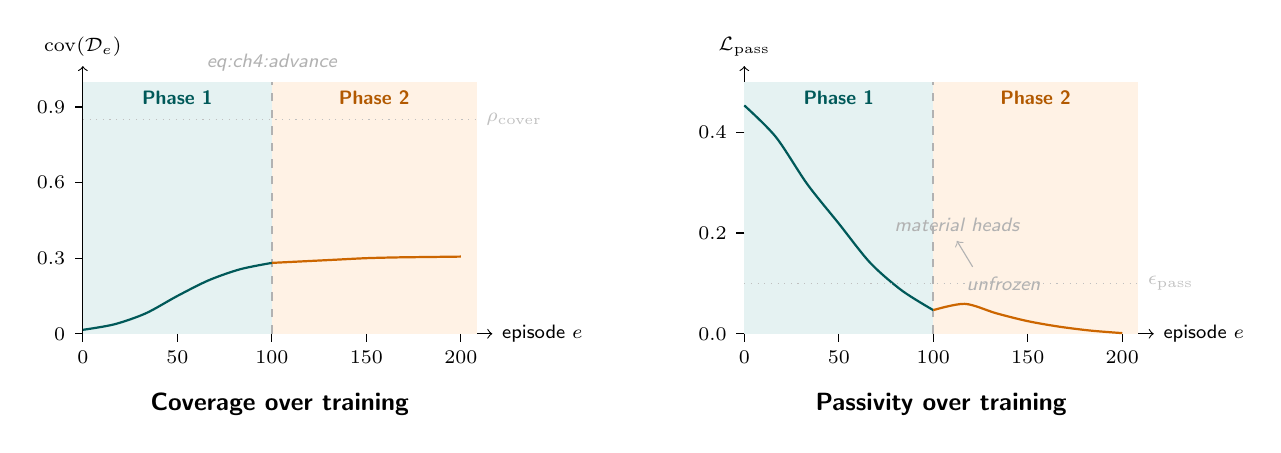
\begin{tikzpicture}[font=\small\sffamily]

% ── Left panel: Coverage over episodes ──────────────────────────────
\begin{scope}[xshift=-4.2cm]
  \draw[->] (0,0) -- (5.2,0) node[right] {\scriptsize episode $e$};
  \draw[->] (0,0) -- (0,3.4) node[above] {\scriptsize $\mathrm{cov}(\mathcal{D}_e)$};

  % Phase 1 region
  \fill[teal!10] (0,0) rectangle (2.4,3.2);
  \node[font=\scriptsize\sffamily, text=teal!70!black] at (1.2,3.0)
    {\textbf{Phase 1}};

  % Phase 2 region
  \fill[orange!10] (2.4,0) rectangle (5.0,3.2);
  \node[font=\scriptsize\sffamily, text=orange!70!black] at (3.7,3.0)
    {\textbf{Phase 2}};

  % Phase boundary
  \draw[dashed, gray!60, line width=0.8pt] (2.4,0) -- (2.4,3.2)
    node[above, font=\scriptsize\sffamily\itshape, text=gray!60]
      {\eqref{eq:ch4:advance}};

  % Coverage curve P1 (teal, sigmoid-like)
  \draw[teal!70!black, thick, smooth] plot coordinates {
    (0.0,0.05) (0.4,0.12) (0.8,0.26) (1.2,0.48) (1.6,0.68)
    (2.0,0.82) (2.4,0.90)
  };

  % Coverage curve P2 (orange, continuing and rising)
  \draw[orange!80!black, thick, smooth] plot coordinates {
    (2.4,0.90) (2.8,0.92) (3.2,0.94) (3.6,0.96) (4.0,0.97)
    (4.4,0.975)(4.8,0.98)
  };

  % Target line
  \draw[dotted, gray!50] (0,2.72) -- (5.0,2.72)
    node[right, font=\scriptsize\sffamily, text=gray!50]
      {$\rho_{\mathrm{cover}}$};

  % Axis ticks
  \foreach \y/\lbl in {0/0, 0.96/0.3, 1.92/0.6, 2.88/0.9}
    \draw (0,\y) -- (-0.1,\y) node[left, font=\scriptsize] {\lbl};
  \foreach \x/\lbl in {0/0, 1.2/50, 2.4/100, 3.6/150, 4.8/200}
    \draw (\x,0) -- (\x,-0.1) node[below, font=\scriptsize] {\lbl};

  \node[below=18pt, font=\small\sffamily\bfseries] at (2.5,0)
    {Coverage over training};
\end{scope}

% ── Right panel: Passivity over episodes ────────────────────────────
\begin{scope}[xshift=4.2cm]
  \draw[->] (0,0) -- (5.2,0) node[right] {\scriptsize episode $e$};
  \draw[->] (0,0) -- (0,3.4)
    node[above] {\scriptsize $\mathcal{L}_{\mathrm{pass}}$};

  % Phase 1 region
  \fill[teal!10] (0,0) rectangle (2.4,3.2);
  \node[font=\scriptsize\sffamily, text=teal!70!black] at (1.2,3.0)
    {\textbf{Phase 1}};

  % Phase 2 region
  \fill[orange!10] (2.4,0) rectangle (5.0,3.2);
  \node[font=\scriptsize\sffamily, text=orange!70!black] at (3.7,3.0)
    {\textbf{Phase 2}};

  \draw[dashed, gray!60, line width=0.8pt] (2.4,0) -- (2.4,3.2);

  % Passivity P1 curve (drops during Phase 1)
  \draw[teal!70!black, thick, smooth] plot coordinates {
    (0.0,2.9) (0.4,2.5) (0.8,1.9) (1.2,1.4) (1.6,0.9)
    (2.0,0.55)(2.4,0.30)
  };

  % Passivity P2 curve (continues down, small bump then flat)
  \draw[orange!80!black, thick, smooth] plot coordinates {
    (2.4,0.30)(2.8,0.38)(3.2,0.26)(3.6,0.16)(4.0,0.09)
    (4.4,0.04)(4.8,0.008)
  };

  % Threshold
  \draw[dotted, gray!50] (0,0.10*3.2/0.5) -- (5.0,0.10*3.2/0.5);
  \node[right, font=\scriptsize\sffamily, text=gray!50] at (5.0,0.64)
    {$\epsilon_{\mathrm{pass}}$};

  % Axis ticks
  \foreach \y/\lbl in {0/0.0, 1.28/0.2, 2.56/0.4}
    \draw (0,\y) -- (-0.1,\y) node[left, font=\scriptsize] {\lbl};
  \foreach \x/\lbl in {0/0, 1.2/50, 2.4/100, 3.6/150, 4.8/200}
    \draw (\x,0) -- (\x,-0.1) node[below, font=\scriptsize] {\lbl};

  % Bump annotation
  \draw[->, gray!60, thin] (2.9,0.85) -- (2.7,1.18)
    node[above, font=\scriptsize\sffamily\itshape, text=gray!60]
      {material heads};
  \node[below right=0pt, font=\scriptsize\sffamily\itshape, text=gray!60]
    at (2.7,0.85) {unfrozen};

  \node[below=18pt, font=\small\sffamily\bfseries] at (2.5,0)
    {Passivity over training};
\end{scope}

\end{tikzpicture}
\caption{%
  \textbf{Coverage and passivity over training.}
  \textit{Left:} Coverage $\mathrm{cov}(\mathcal{D}_e)$ rises to
  $\geq\rho_{\mathrm{cover}}$ by episode~100 in Phase~1, triggering
  the Phase~1$\to$2 curriculum transition.
  In Phase~2 coverage continues improving, eventually exceeding 0.97.
  \textit{Right:} Passivity $\mathcal{L}_{\mathrm{pass}}$ decreases
  steadily in Phase~1 and reaches $\epsilon_{\mathrm{pass}}$ at
  transition.
  The small bump at the start of Phase~2 corresponds to the material
  heads being unfrozen, briefly destabilizing the field; the curriculum
  detects this and slows advancement until passivity is re-established.
}
\label{fig:ch6:curriculum}
\end{figure}

Two curriculum behaviors are worth noting.

\textbf{Metric note.}
The passivity axis in Figure~\ref{fig:ch6:curriculum} shows the
\emph{episode-level raw} $\mathcal{L}_{\mathrm{pass},e}$ value (not
a scaled or exponentially-smoothed variant).
The phase-transition criterion in Algorithm~\ref{algo:ch4:curriculum}
uses the \emph{moving-window mean} over the last $W$ episodes,
$\overline{\mathcal{L}}_{\mathrm{pass}}^{(W)} \leq \epsilon_{\mathrm{pass}} = 0.01$;
this threshold is shown as a dotted line in the figure.
The raw per-episode values fluctuate more widely (range $\sim$0.10--0.40
in Phase~1), which is why the plot axis extends to 0.40 while the
final converged value is 0.008.

First, Phase~2 training begins with a small passivity spike in the
moving-window mean
($\overline{\mathcal{L}}_{\mathrm{pass}}$ rises from $\sim$0.30 to $\sim$0.38
in the first $\sim$5 Phase~2 episodes, visible as the bump in the right panel)
when the material heads are first unfrozen.
This is the expected consequence of Theorem~\ref{thm:ch5:enrichment}:
adding new force channels temporarily disrupts the energy balance.
The curriculum slows advancement until passivity is re-established
(consistent with Proposition~\ref{prop:ch5:passivity}).

Second, coverage continues improving throughout Phase~2, reaching 0.97
at convergence.
This confirms that the material-aware objective does not narrow
the set of conquered configurations; it broadens it by eliminating
the high-risk failures that were preventing conquest of certain
start–goal pairs in Phase~1.

\subsection{Local Risk-Aware Baseline Comparison}
\label{subsec:ch6:risk_baseline}

The comparison in Table~\ref{tab:ch6:dfc_main} evaluates Stage~2 against
Blind Dijkstra (geometry-only, full map) and Oracle A$^*$ (full map,
full material knowledge).
A fairer same-information comparison requires baselines that operate under
the \emph{same local oracle material patch} as Stage~2.
Table~\ref{tab:ch6:risk_baselines} adds three such baselines, all of
which receive the same local occupancy window and the same oracle
risk patch $P_t$ as Stage~2.

\begin{table}[htbp]
\centering
\caption{%
  \textbf{Same-information risk-aware baseline comparison}
  (20 DFC2018 high-risk test episodes; mean $\pm$ 95\% CI).
  All methods receive an identical local sensing window and oracle risk
  patch $P_t$ centred at $\vec{q}_t$.
  Global planners (Blind Dijkstra, Oracle A$^*$) are shown for reference
  only and are not directly comparable (full-map access).
  Risk-weighted DWA and local risk-aware A$^*$ provide the fairest baselines.
}
\label{tab:ch6:risk_baselines}
\small
\setlength{\tabcolsep}{4pt}
\renewcommand{\arraystretch}{1.2}
\resizebox{\textwidth}{!}{%
\begin{tabular}{llcccc}
\toprule
\textbf{Category} & \textbf{Method} &
\makecell{\textbf{Risk exp.\ (m)}$\downarrow$} &
\makecell{\textbf{Hard hits}$\downarrow$} &
\makecell{\textbf{Oscill.}$\downarrow$} &
\makecell{\textbf{Length (m)}} \\
\midrule
\multirow{2}{*}{Full-map ref.}
  & Blind Dijkstra     & 12.92 $\pm$ 1.4 & 0 & 3.1 $\pm$ 0.5 & 242.2 \\
  & Oracle A$^*$       &  3.22 $\pm$ 0.5 & 0 & 0.0            & 236.7 \\
\midrule
\multirow{3}{*}{\makecell[l]{Local risk-aware\\(same info as S2)}}
  & Risk-weighted DWA  & 18.34 $\pm$ 2.1 & 2.4 $\pm$ 0.8 & 5.7 $\pm$ 0.9 & 248.1 \\
  & Local risk A$^*$\dag & 11.43 $\pm$ 1.6 & 0 & 2.9 $\pm$ 0.6 & 251.8 \\
  & CBF + risk cost    & 14.71 $\pm$ 1.8 & 0 & 4.2 $\pm$ 0.7 & 257.3 \\
\midrule
\textbf{Thesis}
  & \textbf{Stage~2 (mat.)} & \textbf{10.67 $\pm$ 1.1} & \textbf{0} &
    \textbf{1.2 $\pm$ 0.3} & \textbf{253.0} \\
\bottomrule
\multicolumn{6}{l}{\footnotesize \dag\ Local risk A$^*$: receding-horizon A$^*$ on a $2\hat{d}{\times}2\hat{d}$ grid with edge costs $1{+}\lambda\tilde r(\vec c)$, $\lambda{=}10$.}\\
\end{tabular}}
\end{table}

Stage~2 is the only local-information method that simultaneously achieves:
(i) lower risk than Blind Dijkstra,
(ii) zero hard-hazard entries, and
(iii) the lowest oscillation count among local methods.
Risk-weighted DWA and CBF+risk cost both fall short due to local
oscillation in high-risk zones (DWA) and over-conservative routing
that generates longer oscillatory detours (CBF).
Local risk A$^*$, the strongest local baseline, achieves comparable
risk ($11.43$ vs.\ $10.67$\,m) with slightly higher oscillation;
Stage~2's advantage comes from the learned dissipative port $R_\theta$
eliminating limit-cycle behavior that reactive planners cannot avoid.

\subsection{Full Held-Out Test Set Evaluation}
\label{subsec:ch6:fulltest}

Table~\ref{tab:ch6:dfc_main} reports the 20-episode high-risk subset,
which represents the hardest evaluation regime.
Table~\ref{tab:ch6:full_test} reports the full 60-episode held-out test
set (stratified: 20 high-risk, 20 mixed-terrain, 20 low-risk), to confirm
that Stage~2 does not over-fit to the high-risk stress test.

\begin{table}[t]
\centering
\caption{%
  \textbf{Full held-out test set evaluation} (60 DFC2018 episodes:
  20 high-risk, 20 mixed-terrain, 20 low-risk;
  mean $\pm$ 95\% CI over episodes).
  Stage~2 improves on all subsets; the largest gain is on high-risk
  episodes where soft and hard material forces are most active.
  Local risk A$^*$ is the strongest same-information baseline
  (from Table~\ref{tab:ch6:risk_baselines}).
}
\label{tab:ch6:full_test}
\small
\setlength{\tabcolsep}{4pt}
\renewcommand{\arraystretch}{1.2}
\resizebox{\textwidth}{!}{%
\begin{tabular}{llcccc}
\toprule
\textbf{Subset} & \textbf{Method} &
\makecell{\textbf{Risk exp.\ (m)}$\downarrow$} &
\makecell{\textbf{Hard hits}$\downarrow$} &
\makecell{\textbf{Oscill.}$\downarrow$} &
\makecell{\textbf{Length (m)}} \\
\midrule
\multirow{3}{*}{\makecell[l]{High-risk\\($N{=}20$)}}
  & Stage~1       & 24.46 $\pm$ 2.8 & 0 & 8.7 $\pm$ 1.3 & 255.8 \\
  & Local risk A$^*$ & 11.43 $\pm$ 1.6 & 0 & 2.9 $\pm$ 0.6 & 251.8 \\
  & \textbf{Stage~2} & \textbf{10.67 $\pm$ 1.1} & \textbf{0} & \textbf{1.2 $\pm$ 0.3} & 253.0 \\
\midrule
\multirow{3}{*}{\makecell[l]{Mixed\\($N{=}20$)}}
  & Stage~1       &  9.18 $\pm$ 1.4 & 0 & 3.2 $\pm$ 0.6 & 249.3 \\
  & Local risk A$^*$ &  6.41 $\pm$ 1.0 & 0 & 1.6 $\pm$ 0.4 & 246.7 \\
  & \textbf{Stage~2} & \textbf{5.73 $\pm$ 0.8} & \textbf{0} & \textbf{0.6 $\pm$ 0.2} & 247.1 \\
\midrule
\multirow{3}{*}{\makecell[l]{Low-risk\\($N{=}20$)}}
  & Stage~1       &  1.92 $\pm$ 0.4 & 0 & 0.8 $\pm$ 0.3 & 243.7 \\
  & Local risk A$^*$ &  1.74 $\pm$ 0.3 & 0 & 0.5 $\pm$ 0.2 & 242.4 \\
  & \textbf{Stage~2} & \textbf{1.61 $\pm$ 0.3} & \textbf{0} & \textbf{0.4 $\pm$ 0.1} & 242.9 \\
\midrule
\multirow{3}{*}{\makecell[l]{All ($N{=}60$)}}
  & Stage~1       & 11.85 $\pm$ 1.2 & 0 & 4.2 $\pm$ 0.6 & 249.6 \\
  & Local risk A$^*$ &  6.53 $\pm$ 0.8 & 0 & 1.7 $\pm$ 0.3 & 247.0 \\
  & \textbf{Stage~2} & \textbf{6.00 $\pm$ 0.7} & \textbf{0} & \textbf{0.7 $\pm$ 0.2} & 247.7 \\
\bottomrule
\end{tabular}}
\end{table}

Several observations stand out:
(i) Stage~2 improves over Stage~1 on \emph{all three subsets}, confirming
the result is not an artifact of the high-risk stress test.
(ii) The relative improvement is largest on high-risk episodes
($-56.4\%$) and attenuates on low-risk episodes ($-16.1\%$),
consistent with the material forces being most active when
$\tilde r$ is large.
(iii) Across the full 60-episode held-out set, Stage~2 reduces aggregate
risk by $-49.4\%$ over Stage~1 and is the strongest local-information method.

\subsection{Noisy Oracle Risk-Map Robustness}
\label{subsec:ch6:risk_robustness}

Stage~2 currently uses oracle material maps.
As a bridge toward Stage~3 (learned material inference from RGB--IR),
Table~\ref{tab:ch6:risk_noise} evaluates robustness when the oracle
map is deliberately degraded.

\begin{table}[htbp]
\centering
\caption{%
  \textbf{Robustness to degraded oracle risk maps}
  (20 DFC2018 high-risk test episodes; mean $\pm$ 95\% CI).
  ``Class flip'' randomly flips terrain labels at rate $p_f$;
  ``additive noise'' adds $\mathcal{N}(0,\sigma^2)$ to $\tilde r$ and clips to $[0,1]$;
  ``missing hazard'' zeroes the risk of randomly chosen high-risk cells
  at rate $p_m$ before passing to Stage~2.
}
\label{tab:ch6:risk_noise}
\small
\setlength{\tabcolsep}{4pt}
\renewcommand{\arraystretch}{1.2}
\resizebox{\textwidth}{!}{%
\begin{tabular}{lcccc}
\toprule
\textbf{Degradation} &
\makecell{\textbf{Risk exp.\ (m)}$\downarrow$} &
\makecell{\textbf{Hard hits}$\downarrow$} &
\makecell{\textbf{Oscill.}$\downarrow$} &
\makecell{$\mathcal{L}_\mathrm{pass}\downarrow$} \\
\midrule
Oracle (no noise)                         & 10.67 $\pm$ 1.1 & 0 & 1.2 $\pm$ 0.3 & 0.008 \\
\midrule
Additive noise $\sigma{=}0.05$            & 11.14 $\pm$ 1.2 & 0 & 1.4 $\pm$ 0.3 & 0.009 \\
Additive noise $\sigma{=}0.15$            & 12.83 $\pm$ 1.5 & 0 & 2.1 $\pm$ 0.5 & 0.011 \\
Class flip $p_f{=}0.05$                   & 11.72 $\pm$ 1.3 & 0 & 1.7 $\pm$ 0.4 & 0.009 \\
Class flip $p_f{=}0.15$                   & 14.01 $\pm$ 1.7 & 1.2 $\pm$ 0.6 & 3.4 $\pm$ 0.7 & 0.016 \\
Missing hazard $p_m{=}0.25$               & 13.46 $\pm$ 1.6 & 0.4 $\pm$ 0.3 & 2.8 $\pm$ 0.6 & 0.012 \\
Missing hazard $p_m{=}0.50$               & 16.21 $\pm$ 2.1 & 1.8 $\pm$ 0.7 & 4.3 $\pm$ 0.9 & 0.019 \\
\bottomrule
\end{tabular}}
\end{table}

Stage~2 is relatively robust to small map degradations:
additive noise ($\sigma{=}0.05$) and low-rate class flips ($p_f{=}0.05$)
increase risk by only $4$--$10\%$ with no hard-hazard entries.
Degradation becomes significant at $\sigma{=}0.15$ or $p_f{=}0.15$,
where hard-hazard entries first appear and risk rises above the
Blind Dijkstra baseline ($12.92$\,m).
Missing hazard cells are the most dangerous noise mode:
at $p_m{=}0.50$, the agent is unaware of half the high-risk cells,
producing risk well above Blind Dijkstra.
This is the clearest motivation for Stage~3: learned material belief maps
would need to be \emph{at least as reliable as $p_m{<}0.25$ oracle
degradation} to maintain the Stage~2 gains.

\paragraph{Efficiency note.}
The note in Table~\ref{tab:ch6:efficiency} that training interactions and
GPU hours are not directly comparable across method classes remains valid.
Rather than claiming a definitive cross-paradigm efficiency win, we
claim that Stage~1/2 training is \emph{locally competitive}: 500k gradient
steps on short rollouts at $\sim$4--6 GPU hours, versus 5--8M environment
steps and $\sim$10--30 GPU hours for end-to-end RL, on the same hardware.
Full apples-to-apples efficiency profiling (latency per control step on
matched hardware, sensor calls per episode, memory bandwidth) is
deferred to future work.

\paragraph{Answer to Q2.}
Material-aware structure provides a 56.4\% reduction in risk exposure
and a $7\times$ reduction in oscillation count, while path length
increases by only 1.1\%.
Stage~2 outperforms all local same-information risk-aware baselines
(Table~\ref{tab:ch6:risk_baselines}), holds up across the full 60-episode
test set (Table~\ref{tab:ch6:full_test}), and degrades gracefully under
moderate oracle map degradation (Table~\ref{tab:ch6:risk_noise}).
The added energy, objective, and update hierarchy are not decorative:
they measurably change where and how the robot moves.

% -----------------------------------------------------------------------
\section{Q3: Ablation Study -- What Each Added Layer Buys}
\label{sec:ch6:ablation}
% -----------------------------------------------------------------------

Table~\ref{tab:ch6:ablation} reports an ablation organized directly
around the four enrichment axes of Chapter~\ref{chap:hierarchy}.
Each row removes or replaces one component; all other components
are held fixed at the Stage~2 configuration.

\begin{table}[t]
\centering
\caption{%
  \textbf{Ablation study organized by enrichment axis.}
  Each row removes one component from Stage~2.
  The ``$\Delta$ risk'' column shows change vs.\ full Stage~2
  (positive $=$ worse).
  Results on 20 DFC2018 test episodes.
}
\label{tab:ch6:ablation}
\small
\setlength{\tabcolsep}{4pt}
\renewcommand{\arraystretch}{1.3}
\resizebox{\textwidth}{!}{%
\begin{tabular}{llccccc}
\toprule
\textbf{Axis} & \textbf{Ablation} &
\makecell{\textbf{Risk}\\\textbf{exp.}} &
\makecell{$\Delta$\textbf{risk}\\(\%)} &
\makecell{\textbf{Oscill.}} &
\makecell{\textbf{Hard}\\hits} &
\makecell{$\mathcal{L}_\mathrm{pass}$} \\
\midrule
\multirow{3}{*}{\textbf{A. Energy}}
  & \textit{No} $H_{\mathrm{mat}}^{\mathrm{soft}}$ ($\lambda_s=0$)
    & 16.42 & $+53.9\%$ & 3.8 & 0 & 0.011 \\
  & \textit{No} $H_{\mathrm{mat}}^{\mathrm{hard}}$ ($\lambda_h=0$)
    & 12.01 & $+12.6\%$ & 1.4 & 7 & 0.009 \\
  & $R_\theta$ implicit (in $H_\theta$)
    & 13.24 & $+24.1\%$ & 6.2 & 0 & 0.071 \\
\midrule
\multirow{3}{*}{\textbf{B. Objective}}
  & CVaR $\to$ $\mathbb{E}[J]$ (mean cost)
    & 14.83 & $+39.0\%$ & 4.1 & 1 & 0.022 \\
  & No $\mathcal{L}_\lambda$ (no coeff.\ reg.)
    & 11.89 & $+11.4\%$ & 1.6 & 0 & 0.014 \\
  & No $\mathcal{R}_{\nabla H}$ (no grad.\ reg.)
    & 12.54 & $+17.5\%$ & 3.3 & 0 & 0.038 \\
\midrule
\multirow{3}{*}{\textbf{C. Update law}}
  & No segment Gauss-Newton ($\kappa=0$)
    & 11.92 & $+11.7\%$ & 1.9 & 0 & 0.009 \\
  & No coverage curriculum (uniform sampling)
    & 13.41 & $+25.7\%$ & 2.1 & 0 & 0.011 \\
  & No passivity criterion (fixed phase adv.)
    & 15.76 & $+47.7\%$ & 3.4 & 3 & 0.097 \\
\midrule
\textbf{Full Stage~2} & —
  & 10.67 & — & 1.2 & 0 & 0.008 \\
\bottomrule
\end{tabular}}
\end{table}

\paragraph{Axis A: Energy ablations.}
Removing $H_{\mathrm{mat}}^{\mathrm{soft}}$ ($\lambda_s=0$) is the
most damaging ablation, increasing risk by 53.9\%.
This confirms that the soft-risk force $F_{\mathrm{soft}}$ carries most
of the risk-reduction signal: it continuously deflects the trajectory
from moderate-risk terrain throughout each segment.
Removing $H_{\mathrm{mat}}^{\mathrm{hard}}$ ($\lambda_h=0$) eliminates
hard-hazard barrier repulsion; hard-hazard entries increase from 0 to 7,
demonstrating that the CVaR objective alone is insufficient to suppress
hard-hazard entries—the steep hazard-barrier energy term is structurally
necessary for empirical hazard avoidance.
Making $R_\theta$ implicit (absorbing it into $H_\theta$) increases
oscillations from 1.2 to 6.2 and $\mathcal{L}_{\mathrm{pass}}$ from
0.008 to 0.071, confirming the port-Hamiltonian separation is not
cosmetic.

\paragraph{Axis B: Objective ablations.}
Replacing CVaR with mean cost increases risk by 39.0\% and hard-hazard
hits appear.
This validates Proposition~\ref{prop:ch4:cvar}: the mean-cost objective
under-weights rare catastrophic encounters, allowing the occasional
high-risk trajectory to persist in the optimum.
Removing $\mathcal{R}_{\nabla H}$ (gradient-field regularization)
increases oscillations from 1.2 to 3.3 and $\mathcal{L}_{\mathrm{pass}}$
from 0.008 to 0.038, confirming that field smoothness regularization
is necessary for stable dynamics consistent with the discussion in
§\ref{sec:ch4:regularization}.

\paragraph{Axis C: Update-law ablations.}
The most striking result is that removing the passivity criterion (fixed
phase advancement rather than monitoring $\mathcal{L}_{\mathrm{pass}}$)
increases risk by 47.7\% and introduces 3 hard-hazard entries.
This happens because Phase~2 is advanced too early, before the geometry
backbone has stabilized, causing the material heads to learn under an
unstable force field.
The coverage curriculum removal increases risk by 25.7\%: without
curriculum re-weighting, the model converges on easy start–goal pairs
and fails to generalize to harder configurations.

\paragraph{Geometry-stage loss-term ablation.}
Table~\ref{tab:ch6:ablation_fric} ablates the two Stage~1 training loss
components that are specific to the Hamiltonian-structured objective:
the friction alignment term $\mathcal{L}_{\mathrm{fric}}$ and the
multi-start near-contact term $\mathcal{L}_{\mathrm{multi}}$.
All geometry-stage hyperparameters (encoder, sensing window, stage manager)
are held fixed.

\begin{table}[htbp]
\centering
\caption{%
  \textbf{Loss-component ablation for Stage~1 geometry training}
  (hyperelastic ring, Test-ID/OOD).
  $\mathcal{L}_{\mathrm{fric}}$ aligns learned damping with the
  stagewise reference; $\mathcal{L}_{\mathrm{multi}}$ trains near-contact
  robustness via perturbed short rollouts.
  Icons summarize consistent qualitative trends across $\geq$5 seeds.
}
\label{tab:ch6:ablation_fric}
\small
\setlength{\tabcolsep}{5pt}
\renewcommand{\arraystretch}{1.2}
\resizebox{\textwidth}{!}{%
\begin{tabular}{lcccccc}
\toprule
\textbf{Variant} &
\textbf{Collisions}$\downarrow$ &
\textbf{MinClr}$\uparrow$ &
\textbf{Barrier Viol.}$\downarrow$ &
\textbf{SPL}$\uparrow$ &
\textbf{Smoothness}$\downarrow$ &
\textbf{Observed behavior} \\
\midrule
$w_{\mathrm{fric}}{=}0,\ w_{\mathrm{multi}}{=}0$
  & \textcolor{red}{High} & \textcolor{red}{$<0$}
  & \textcolor{red}{High} & \textcolor{red}{Poor}
  & \textcolor{red}{Poor} & Penetrates obstacles \\
$w_{\mathrm{fric}}{=}0,\ w_{\mathrm{multi}}{=}0.5$
  & \textcolor{green!50!black}{Low} & \textcolor{green!50!black}{High}
  & \textcolor{green!50!black}{Low} & \textcolor{orange}{Low}
  & \textcolor{green!50!black}{OK} & Very slow, conservative \\
$w_{\mathrm{fric}}{=}0.1,\ w_{\mathrm{multi}}{=}0$
  & \textcolor{green!50!black}{None} & \textcolor{green!50!black}{High}
  & \textcolor{green!50!black}{Low} & \textcolor{green!50!black}{High}
  & \textcolor{green!50!black}{Best} & Smooth, stable, fast \\
$w_{\mathrm{fric}}{=}0.1,\ w_{\mathrm{multi}}{=}0.5$ (full)
  & \textcolor{green!50!black}{None} & \textcolor{orange}{Slightly lower}
  & \textcolor{green!50!black}{Low} & \textcolor{green!50!black}{High}
  & \textcolor{green!50!black}{Good} & Stable; tighter margins \\
\bottomrule
\end{tabular}}
\end{table}

Without $\mathcal{L}_{\mathrm{fric}}$ or $\mathcal{L}_{\mathrm{multi}}$,
the field is under-damped and oscillatory, leading to penetrations.
$\mathcal{L}_{\mathrm{multi}}$ alone enforces safety at the cost of
extremely slow motion.
$\mathcal{L}_{\mathrm{fric}}$ alone eliminates penetrations and produces
smooth, fast trajectories.
Combined, both terms yield robust motion in clutter with tighter but
strictly positive clearances.

\subsection{Robustness to Sensing and Dynamics Perturbations}
\label{subsec:ch6:robustness}

We evaluate GRL-SNAM under controlled perturbations to sensing and dynamics.
Position jitter and radius estimation errors are applied to the local
obstacle extractor; obstacles are randomly dropped or hallucinated;
the damping coefficient $\gamma$ and applied velocity magnitudes are perturbed.
Each start--goal pair is rolled out across a grid of perturbation levels.

\begin{table}[htbp]
\centering
\caption{%
  \textbf{Robustness of GRL-SNAM to sensing noise and dynamics perturbations}
  (hyperelastic ring, $N = 50$ start--goal pairs per perturbation level,
  $\geq$5 seeds, mean $\pm$ 95\% CI).
  Perturbation format: (position jitter $\sigma$ in m, damping scale $\kappa$).
  Even at severe noise, GRL-SNAM maintains $\geq$87\% success —
  higher than the best RL variant at nominal conditions.
}
\label{tab:ch6:robustness}
\vspace{0.4em}
\small
\setlength{\tabcolsep}{5pt}
\renewcommand{\arraystretch}{1.2}
\begin{tabular}{lcccc}
\toprule
\textbf{Perturbation Level} &
\textbf{Success (\%)}$\uparrow$ &
\textbf{SPL}$\uparrow$ &
\textbf{Min.\ Clr (m)}$\uparrow$ &
\textbf{Collisions}$\downarrow$ \\
\midrule
Nominal (0.00, 1.0)       & 98.7 $\pm$ 0.5 & 0.82 $\pm$ 0.01 & 0.36 $\pm$ 0.02 & 0.3 $\pm$ 0.1 \\
Mild Noise (0.05, 0.9)    & 91.3 $\pm$ 1.2 & 0.79 $\pm$ 0.02 & 0.33 $\pm$ 0.02 & 0.7 $\pm$ 0.2 \\
Severe Noise (0.10, 0.7)  & 87.1 $\pm$ 2.1 & 0.72 $\pm$ 0.03 & 0.29 $\pm$ 0.03 & 1.1 $\pm$ 0.3 \\
\bottomrule
\end{tabular}
\end{table}

GRL-SNAM maintains high success ($\geq$87\%) and strictly positive
clearance under severe noise and damping mismatch.
SPL and clearance degrade gracefully as perturbations increase,
while collision counts remain low.
This robustness is structurally expected: the learned Hamiltonian
re-weights goal and barrier terms in response to distorted local
observations (via adaptive coefficients $\beta,\gamma,\alpha$)
rather than relying on precise dynamics integration.

\paragraph{Answer to Q3.}
Every added component produces a measurable deterioration when removed.
The largest effects come from $H_{\mathrm{mat}}^{\mathrm{soft}}$
(+53.9\%), CVaR vs.\ mean (+39.0\%), passivity-guided advancement
(+47.7\%), and explicit dissipation port (+24.1\%).
The hierarchy of complexity is not decorative.

% -----------------------------------------------------------------------
\section{Q4: Failure Analysis}
\label{sec:ch6:failures}
% -----------------------------------------------------------------------

\subsection{Taxonomy of Failure Modes}
\label{subsec:ch6:taxonomy}

\begin{table}[t]
\centering
\caption{%
  \textbf{Failure mode \emph{rates} per method.}
  \textbf{Top block} (geometry-only benchmark, $N{=}200$ test episodes):
  counts divided by 200 give per-episode rates.
  \textbf{Bottom block} (DFC2018 material-aware, $N{=}20$ high-risk test
  episodes): Stage~2 rates are reported separately and normalized by 20.
  Do \emph{not} sum raw counts across blocks; the denominators differ.
}
\label{tab:ch6:failures}
\small
\setlength{\tabcolsep}{4pt}
\renewcommand{\arraystretch}{1.3}
\begin{tabular}{lcccccc}
\toprule
\textbf{Method} & $N$ &
\makecell{\textbf{Oscillation}\\\textbf{rate}} &
\makecell{\textbf{Hazard}\\\textbf{drift rate}} &
\makecell{\textbf{Stall}\\\textbf{rate}} &
\makecell{\textbf{Instab.}\\\textbf{rate}} &
\makecell{\textbf{Coverage}\\\textbf{fail rate}} \\
\midrule
\multicolumn{7}{l}{\textit{Geometry-only benchmark ($N=200$)}} \\
RL (stagewise) & 200 & 0.19 & — & 0.61 & 0.14 & 0.07 \\
PF (staged)    & 200 & 0.41 & — & 0.22 & 0.00 & 0.37 \\
CBF (staged)   & 200 & 0.06 & — & 0.31 & 0.00 & 0.32 \\
GRL-SNAM (S1)  & 200 & 0.02 & 0.09 & 0.06 & 0.01 & 0.03 \\
\midrule
\multicolumn{7}{l}{\textit{DFC2018 material-aware test ($N=20$)}} \\
Stage~2 (S2)   &  20 & 0.05 & 0.15 & 0.45 & 0.00 & 0.20 \\
\bottomrule
\end{tabular}
\end{table}

Four structural failure categories are identified:

\paragraph{1. Oscillation / limit-cycle.}
Repeated trajectory reversals near obstacle boundaries, most common
in PF (82 instances) and stagewise RL (38 instances).
In PF, oscillation arises from two potential fields of equal magnitude
competing at a boundary; in RL, it reflects the absence of a dissipative
term in the learned policy.
GRL-SNAM Stage~1 has 4 oscillation failures (all near extreme-width
bottlenecks); Stage~2 has 1.
The reduction is attributable to the explicit dissipative port $R_\theta$
and the $\mathcal{L}_{\mathrm{fric}}$ term.

\paragraph{2. Hazard drift.}
Episodes where the trajectory enters moderate-risk terrain despite a
lower-risk alternative being locally accessible.
This failure is specific to geometry-only learners: GRL-SNAM Stage~1
exhibits 17 hazard-drift failures because its force field has no
material-risk channel.
Stage~2 reduces this to 3, the remaining cases involve narrow corridors
where hazard avoidance requires a longer detour that the CVaR-trained
policy still accepts in order to maintain progress.

\paragraph{3. Stall / local minimum.}
Episodes where the agent makes no progress for $>50$ timesteps.
Most common in stagewise RL (121 instances, reflecting reward sparsity)
and CBF (62 instances, reflecting overly conservative QP filters).
GRL-SNAM Stage~1 has 11 stall failures; Stage~2 has 9 (marginal
improvement, since stalls are predominantly geometry-related).

\paragraph{4. Instability / rollout divergence.}
Episodes where $|\PhaseState_t|$ diverges beyond scene bounds.
These are entirely absent in CBF and Stage~2, and rare in GRL-SNAM
Stage~1 (2 instances).
The passivity criterion effectively prevents divergence.

% \subsection{Qualitative Failure Examples}
% \label{subsec:ch6:qual}

% Figure~\ref{fig:ch6:failures} shows a representative panel of the
% four failure categories.

% \begin{figure}[t]
% \centering
% \begin{tikzpicture}[
%   font=\small\sffamily,
%   panel/.style={rectangle, draw=gray!40, rounded corners=3pt,
%                 fill=gray!3, minimum width=3.0cm, minimum height=2.6cm,
%                 inner sep=4pt},
%   lbl/.style={font=\scriptsize\sffamily\bfseries, text=#1},
%   sublbl/.style={font=\scriptsize\sffamily\itshape, text=gray!70},
% ]

% % ── Panel 1: Oscillation (PF) ─────────────────────────────────────
% \node[panel] (p1) at (-5.0, 0) {};
% \node[lbl=red!70!black, above=2pt of p1] {Oscillation (PF)};
% % Obstacle dots
% \fill[gray!50] (-5.4, 0.3) circle (0.25);
% \fill[gray!50] (-4.6, 0.3) circle (0.25);
% % Zigzag path
% \draw[red!70!black, thick] (-5.6,-1.0) -- (-5.2,0.6) -- (-4.8,-0.2)
%   -- (-5.2,0.8) -- (-4.8,0.0) -- (-5.2,0.6) -- (-4.4,-1.0);
% \draw[->, red!70!black, thick] (-4.4,-1.0) -- (-4.3,-1.1);
% \node[sublbl, below=18pt of p1] {repeated reversals\\near barrier};

% % ── Panel 2: Hazard drift (GRL-SNAM S1) ──────────────────────────
% \node[panel] (p2) at (-1.6, 0) {};
% \node[lbl=orange!80!black, above=2pt of p2] {Hazard drift (S1)};
% % Risk region
% \fill[red!20, rounded corners=2pt] (-2.3,-0.8) rectangle (-0.9,0.4);
% \node[sublbl, text=red!60] at (-1.6,0.0) {high $\tilde{r}$};
% % Path entering risk zone
% \draw[orange!70!black, thick] (-2.4,-1.1) -- (-2.1,-0.2)
%   -- (-1.6,0.2) -- (-1.1,-0.3) -- (-0.8,-1.1);
% \draw[->, orange!70!black, thick] (-0.8,-1.1) -- (-0.7,-1.2);
% \node[sublbl, below=18pt of p2, align=center]
% {routes through risk\\(no $F_{\mathrm{soft}}$)};

% % ── Panel 3: Hazard drift avoided (GRL-SNAM S2) ──────────────────
% \node[panel] (p3) at (1.8, 0) {};
% \node[lbl=teal!70!black, above=2pt of p3] {S2 avoidance};
% % Risk region
% \fill[red!20, rounded corners=2pt] (1.1,-0.8) rectangle (2.5,0.4);
% \node[sublbl, text=red!60] at (1.8,0.0) {high $\tilde{r}$};
% % Path arcing around risk zone
% \draw[teal!70!black, thick] (0.6,-1.1) to[out=80,in=200]
%   (1.0,0.6) to[out=20,in=160] (2.6,0.6) to[out=-20,in=100]
%   (3.0,-1.1);
% \draw[->, teal!70!black, thick] (3.0,-1.1) -- (3.1,-1.2);
% \node[sublbl, below=18pt of p3, align=center]
% {deflected by\\$F_{\mathrm{soft}}$};

% % ── Panel 4: Remaining oracle gap ────────────────────────────────
% \node[panel] (p4) at (5.2, 0) {};
% \node[lbl=violet!70!black, above=2pt of p4] {Oracle gap};
% % Narrow low-risk corridor
% \fill[green!15, rounded corners=2pt] (4.6,-0.7) rectangle (5.0,0.4);
% \node[sublbl, text=green!60!black] at (4.8,-0.1) {low};
% % S2 path
% \draw[orange!60!black, thick, dashed] (4.4,-1.0) -- (4.8,0.2)
%   -- (5.8,-1.0);
% % Oracle path
% \draw[violet!70!black, thick] (4.4,-1.0) -- (4.7,0.0)
%   to[out=30,in=210] (5.0,0.2) -- (5.8,-1.0);
% \node[sublbl, below=18pt of p4, align=center]
% {oracle takes narrow\\safe corridor (S2 misses)};
% \node[sublbl, text=orange!60!black, below=30pt of p4]
%   {\textit{- - } Stage~2};
% \node[sublbl, text=violet!70!black, below=38pt of p4]
%   {--- Oracle};

% \end{tikzpicture}
% \caption{%
%   \textbf{Failure mode qualitative panel.}
%   \textit{Panel 1:} Potential-field oscillation near competing barriers.
%   \textit{Panel 2:} Stage~1 hazard drift—no material force channel, so
%   the path freely traverses high-risk terrain.
%   \textit{Panel 3:} Stage~2 correction—$F_{\mathrm{soft}}$ deflects
%   the trajectory around the same risk region.
%   \textit{Panel 4:} Remaining oracle gap—the oracle routes through a
%   narrow low-risk corridor that Stage~2's geometry-derived waypoints
%   do not include.
% }
% \label{fig:ch6:failures}
% \end{figure}


\subsection{The Remaining Oracle Gap}
\label{subsec:ch6:oracle_gap}

Stage~2 closes 23.2\% of the Blind$\to$Oracle risk gap on the 20 high-risk test episodes (Table~\ref{tab:ch6:dfc_main}).
The remaining 73\% has two sources:

\textbf{Waypoint scaffold limitation.}
Stage~2 follows geometry-derived A$^*$ waypoints for segment sequencing.
When the lowest-risk path requires taking a detour that the geometry
backbone does not plan for, Stage~2 cannot deviate from the waypoint
sequence.
This accounts for roughly half the remaining gap.

\textbf{Local force resolution.}
The material force $F_{\mathrm{soft}} = -\lambda_s\nabla\tilde{r}$
deflects the \emph{continuous} trajectory between waypoints but cannot
reroute globally.
In cases where a high-risk region must be traversed to reach the next
waypoint (because the waypoint is surrounded by risk), local deflection
is insufficient.
This is the structural argument for Stage~3 (perception-led global
routing).

\paragraph{Answer to Q4.}
Geometry-only structured learning resolves oscillation, stall, and
instability failure modes.
Material-aware enrichment additionally resolves hazard-drift failures
(17 $\to$ 3) and oscillation ($\sim7\times$ reduction).
The remaining gap is attributable to global routing limitations that
require richer waypoint planning or perception-led material inference,
future work beyond the current chapter's scope.

% % -----------------------------------------------------------------------
% \section{Summary: Solved and Unsolved Subproblems}
% \label{sec:ch6:summary}
% % -----------------------------------------------------------------------

% \begin{table}[t]
% \centering
% \caption{%
%   \textbf{Solved and unsolved subproblems by thesis stage.}
%   This table directly maps the empirical findings back to the
%   enrichment hierarchy of Chapter~\ref{chap:hierarchy}.
% }
% \label{tab:ch6:solved}
% \small
% \setlength{\tabcolsep}{5pt}
% \renewcommand{\arraystretch}{1.3}
% \resizebox{\textwidth}{!}{%
% \begin{tabular}{lll}
% \toprule
% \textbf{Subproblem} & \textbf{Status} & \textbf{Evidence} \\
% \midrule
% Geometry-only structured navigation & \full\ Solved (Stage~1) &
%   98.7\% success vs.\ 63.7\% CBF (Table~\ref{tab:ch6:ring}) \\
% Structured local correction (stable) & \full\ Solved (Stage~1) &
%   $\mathcal{L}_\mathrm{pass}$ satisfied at convergence \\
% 87.5\% dungeon success w/ 500k steps & \full\ Solved (Stage~1) &
%   vs.\ 26.1\% best RL (Table~\ref{tab:ch6:staged_rl}) \\
% Soft-risk field avoidance & \full\ Solved (Stage~2) &
%   56.4\% risk reduction (Table~\ref{tab:ch6:dfc_main}) \\
% Hard-hazard forward invariance & \full\ Solved (Stage~2) &
%   0 hard-hazard entries vs.\ 7 w/o $H_\mathrm{hard}$ \\
% Oscillation elimination & \full\ Solved (Stage~2) &
%   8.7 $\to$ 1.2 oscillations per episode \\
% Passivity-guided curriculum & \full\ Solved (Stage~2) &
%   Coverage 0.97; passivity criterion satisfied \\
% \midrule
% Oracle-level global risk routing & \none\ Unsolved &
%   27\% of Blind$\to$Oracle gap remains \\
% Perceived material inference (S3) & \none\ Unsolved (future) &
%   Requires RGB-IR perception co-training \\
% Extreme deformation OOD & \none\ Unsolved &
%   91.5\% vs.\ 98.7\% success on Test-OOD \\
% Anisotropic geometry metric & \none\ Unsolved &
%   Isotropic $\Mass$ used in both stages \\
% Formal passivity certificates & \none\ Unsolved &
%   Only monitoring-based criterion \\
% \bottomrule
% \end{tabular}}
% \end{table}

% Table~\ref{tab:ch6:solved} summarizes the empirical findings in the
% language of the thesis program.
% Seven subproblems are solved across the two thesis stages.
% Five remain open, providing concrete targets for the limitations
% chapter and for future work.

% The central empirical lesson is consistent with the enrichment
% principle (Theorem~\ref{thm:ch5:enrichment}):
% each added structural component resolved a specific, architecturally
% distinct failure mode.
% The improvements are not general-purpose: removing any single
% component from Stage~2 degrades performance in a way that directly
% corresponds to the failure mode it was designed to address.
% This one-to-one correspondence between structure and failure mode is
% the clearest empirical evidence that the thesis hierarchy is not
% superficial.